\subsubsection{Selección del perfil de movimiento horizontal}
Se selecciona un perfil de aluminio V-Slot con ruedas de precisión, que ofrece:
\begin{itemize}[label=$\bullet$]
    \item Capacidad de carga de hasta 50\,kg
    \item Sistema de ajuste para eliminación de juego mecánico
    \item Alta precisión de movimiento
\end{itemize}

Cálculo de deflexión \\
\noindent
Para verificar la rigidez del perfil, se analiza como una viga simplemente apoyada bajo carga centrada:
\begin{equation}
\delta = \frac{F \cdot L^3}{48 \cdot E \cdot I}
\label{eq:deflexion_perfil}
\end{equation}

donde:
\begin{itemize}[label=$\bullet$]
    \item $E = 69\,000$\,N/mm$^2$ (módulo de Young del aluminio)
    \item $L = 3\,000$\,mm (longitud del perfil)
    \item $I$ = momento de inercia del perfil
    \item $F$ = carga aplicada
\end{itemize}

Para un perfil V-Slot 20$\times$80\,mm, con $I = 350\,000$\,mm$^4$, la deflexión calculada es:
\[\delta = 0.87\,\text{mm}\]

Este valor es aceptable considerando que representa menos del 0.03\% de la longitud total del perfil, cumpliendo con criterios de rigidez para aplicaciones de precisión moderada.

Como complemento, se seleccionan dos carros lineales estándar de 100\,mm de ancho, cada uno equipado con 4 ruedas tipo DELRIN que se desplazan sobre el perfil V-Slot.
\begin{figure}[H]
    \centering
    \begin{subfigure}{0.35\textwidth}
        \centering
        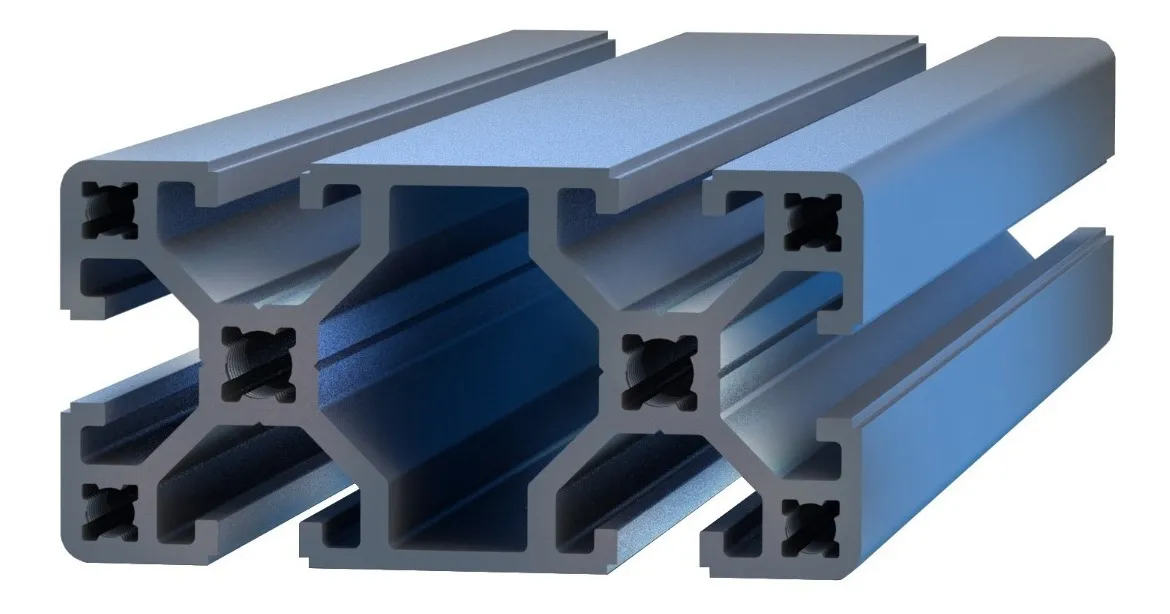
\includegraphics[width=0.7\textwidth]{img/vslot_40x80.png}
        \caption{\textit{Perfil v-slot.}}
        \label{fig:vslot_40x80}
    \end{subfigure}
    \hspace{0.5cm}
    \begin{subfigure}{0.35\textwidth}
        \centering
        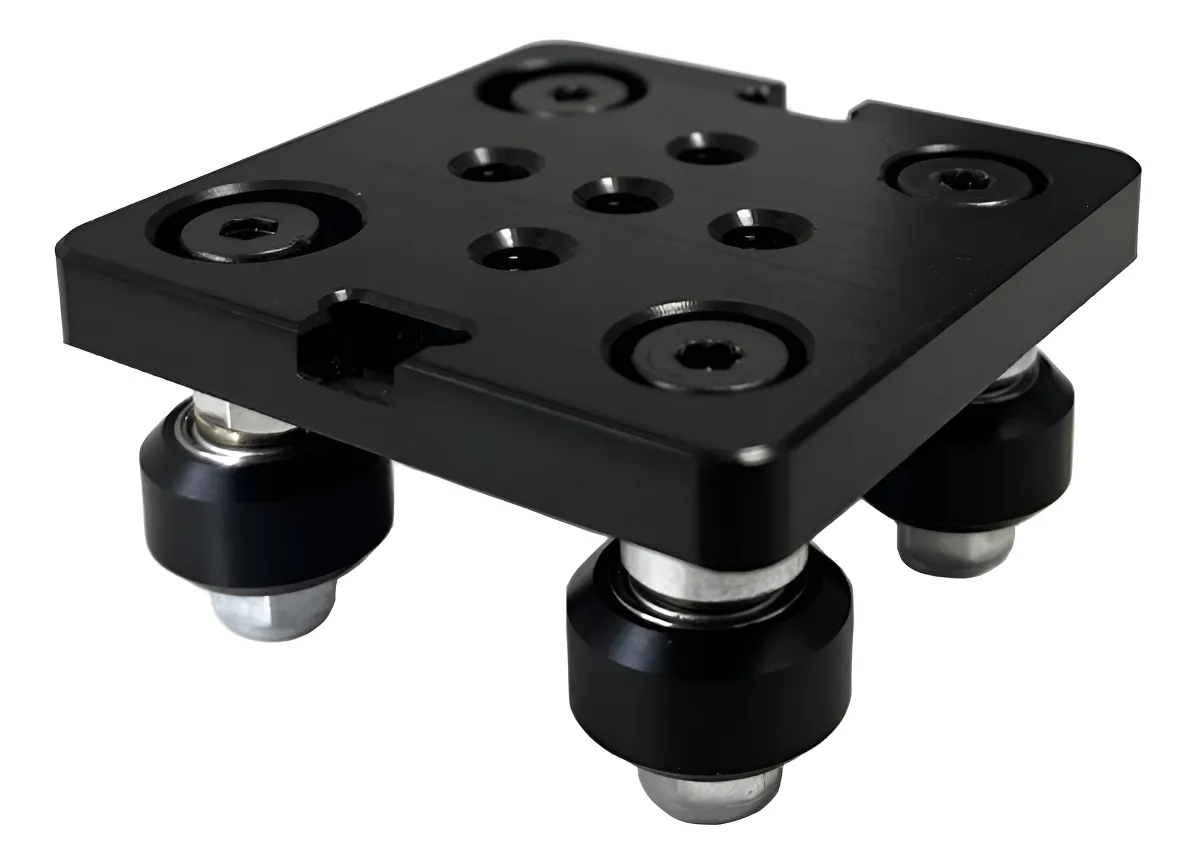
\includegraphics[width=0.4\textwidth]{img/carro_perfilvslot.png}
        \caption{\textit{Sistema de ruedas para deslizamiento sobre perfil v-slot.}}
        \label{fig:carro_perfilvslot}
    \end{subfigure}
    \caption{\textit{Sistema de deslizamiento con perfil v-slot.}}
\end{figure}
Al activarse los motores del robot serie se genera una fuerza F1 como la que se muestra en \ref{fig:esfuerzo_lateral}. Dicha fuerza genera que toda la estructura vertical se mueva hacia atras.
\begin{figure}[H]
        \centering
        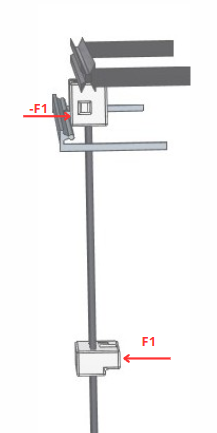
\includegraphics[width=0.3\textwidth]{img/esfuerzo_lateral.png}
        \caption{\textit{Analisis cualitativo de fuerzas.}}
        \label{fig:esfuerzo_lateral}
\end{figure}
Para eliminar ese movimiento se coloca un perfil como el de la fig \ref{fig:barra_lateral}, en conjunto con sus rodamientos (fig. \ref{fig:sbr20uu}) acoplados al soporte superior. De esta manera se genera una fuerza semejante a F1 pero en sentido contrario.
\begin{figure}[H]
    \centering
    \begin{subfigure}{0.35\textwidth}
        \centering
        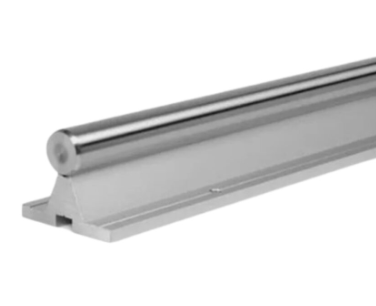
\includegraphics[width=0.7\textwidth]{img/barra_lateral.png}
        \caption{\textit{Barra lateral.}}
        \label{fig:barra_lateral}
    \end{subfigure}
    \hspace{0.5cm}
    \begin{subfigure}{0.35\textwidth}
        \centering
        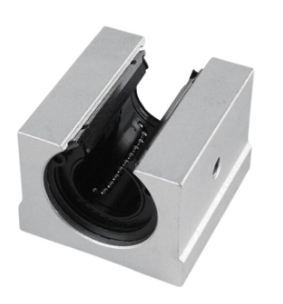
\includegraphics[width=0.65\textwidth]{img/sbr20uu.png}
        \caption{\textit{Carro para deslizamiento sobre barra lateral.}}
        \label{fig:sbr20uu}
    \end{subfigure}
    \caption{Sistema de rigidez horizontal.}
\end{figure}


\subsubsection{Sistema de transmisión por correa}
El sistema utiliza correa dentada GT2 con poleas de igual diámetro en ambos extremos. La longitud de correa necesaria se calcula como:
\begin{equation}
L = 2C + \pi D = 6.06\,\text{m}
\label{eq:longitud_correa}
\end{equation}
donde $C$ es la distancia entre centros de las poleas y $D$ el diámetro de las mismas. \\

Distribución de cargas en el sistema\\
\noindent
La carga total de 12.72\,kg se distribuye entre dos subsistemas mecánicos:

\begin{itemize}[label=$\bullet$]
    \item \underline{Carga soportada por el perfil V-Slot:} El perfil y los carros lineales soportan directamente el peso vertical de la carga (8.96\,kg) a través de las ruedas DELRIN. Esta carga genera únicamente esfuerzos de compresión y flexión en el perfil, sin afectar directamente al sistema de transmisión.
    
    \item \underline{Carga dinámica del motor:} El motor debe vencer las fuerzas necesarias para acelerar y mover horizontalmente la masa efectiva del sistema (12.72\,kg).
\end{itemize}

Esta distribución asume un coeficiente de fricción por rodadura de $\mu_{\text{rod}} \approx 0.001$ para ruedas DELRIN sobre aluminio.\\ \\
Selección polea y correa\\
\noindent
Se selecciona una polea GT2 de 40 dientes y diametro de 25.5mm que tiene 80mm/rev

\begin{enumerate}
    \item \underline{Precisión de posicionamiento}: El desplazamiento lineal por revolución determina la resolución del sistema:
    \begin{equation}
    \text{Resolución} = \frac{P}{n_{\text{pasos/rev}}} = 0.05mm/paso
    \end{equation}
    donde P=80mm/rev, $n_{\text{pasos/rev}} = 200 \times 8 = 1600$ pasos (con 8 micropasos). Esto implica 20 pasos/mm.
    \item \underline{Velocidad de operación}: Para una velocidad lineal objetivo de $v_{\text{max}} = 250$\,mm/s, la velocidad angular requerida es:
    \begin{equation}
    n = \frac{v_{\text{max}}}{P} \times 60 = 187.5 [\text{RPM}] 
    \end{equation}
    Velocidad que se encuentra en la zona de torque máximo.
\end{enumerate}
Para esta polea, se selecciona una correa dentada de 10mm de ancho.\\

Análisis de fuerzas\\
Para determinar el torque motor requerido, se consideran las siguientes fuerzas resistivas:

\begin{enumerate}
    \item \underline{Fricción por rodadura:}
    \begin{equation}
    F_{\text{rod}} = \mu_{\text{rodadura}} \cdot m \cdot g \cdot \frac{1}{r_{\text{rueda}}}= 0.021N
    \end{equation}
    donde $\mu_{\text{rodadura}}$ depende del material de las ruedas DELRIN sobre aluminio.
    
    \item \underline{Fuerza de aceleración:}
    \begin{equation}
    F_{\text{acel}} = (m_{\text{carga}} + m_{\text{correa}}) \cdot a_{\text{max}} = 2.43 N
    \end{equation}
    Incluye la masa de la carga útil y la masa lineal de la correa GT2.
    
    \item \underline{Fricción en rodamientos de poleas:}
    \begin{equation}
    F_{\text{friccion\_rod}} = T_{\text{correa}} \cdot \mu_{\text{rodamientos}} \cdot n = 0.12N
    \end{equation}
    con $n = 2$ (polea conducida y tensor).
    
    \item \underline{Fuerza interna de la correa:}
    \begin{equation}
    F_{\text{correa}} = 0.5\,\text{N}
    \end{equation}
    Valor empírico para correas GT2 según especificaciones del fabricante.
    
    \item \underline{Otras pérdidas:}
    \begin{equation}
    F_{\text{otras}} = 0.1 \cdot (F_{\text{acel}} + F_{\text{rod}})=0.26N
    \end{equation}
    Se estima un 10\% adicional para pérdidas no modeladas.
\end{enumerate}

Cálculo del torque motor\\
Considerando la distribución de cargas analizada anteriormente, donde el motor debe mover la masa total (12.72\,kg), la fuerza total requerida en la base del sistema es:
\begin{equation}
F_{\text{tbase}} = 3.33\,\text{N}
\end{equation}


Aplicando un factor de seguridad de 2.5 para contemplar condiciones adversas de operación y degradación del sistema con el uso, el torque motor necesario resulta:
\begin{equation}
T_{\text{motor}} = F_{\text{tbase}} \cdot 2.5 \cdot r_{\text{polea}} \approx 0.1\,\text{Nm}
\label{eq:torque_motor}
\end{equation}

Selección del motor\\
Se selecciona un motor paso a paso NEMA 17. Analizando la curva dinámica torque-velocidad (Figura~\ref{fig:Curva_din_nema34}), se verifica que para la velocidad máxima de operación de 250\,mm/s (187.5\,rpm), el torque disponible supera ampliamente el requerimiento calculado de 0.1\,Nm, garantizando un margen de seguridad adecuado para la operación continua del sistema. 
\begin{figure}[H]
    \centering
    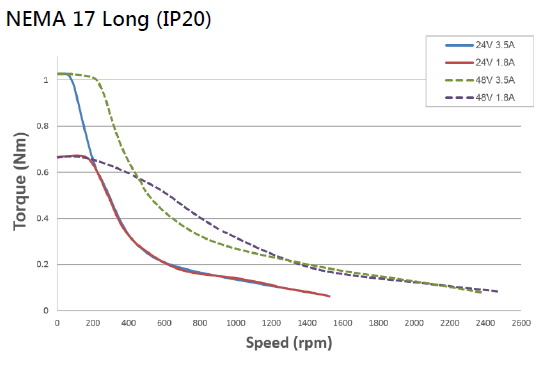
\includegraphics[width=0.65\textwidth]{img/Nema17.png}
    \caption{\textit{Curva dinámica torque-velocidad del motor paso a paso NEMA 17.}}
    \label{fig:Curva_din_nema17}
\end{figure}